%styles
%Da Latex für englischsprachige Texte ausgerichtet ist,
%wird als Dokumentenklasse das "`scrbook"' von Markus Kohm verwendet.
%Dieses ist für deutschsprachige Texte ausgelegt.
%BCOR12mm: 12mm Bindekorrektur (Verbreiterung des linken Randes)
%DIV11: entspricht in etwas der geforderten Textgröße und Seitenränder
%titlepage: eine Titelseite wird verwendet
%a4paper: DIN A4
%oneside: für eine spätere einseitige Bedruckung
\documentclass[BCOR12mm,DIV11,titlepage,a4paper,oneside,10pt]{scrbook}


% Farben definieren
\usepackage{color}
\usepackage[html]{xcolor}
\definecolor{m_green}{HTML}{00AD2F}
%\definecolor{m_pink}{HTML}{D40B6F}
\definecolor{m_pink}{HTML}{dd1166}
\definecolor{m_grey}{HTML}{555555}
\definecolor{m_lila}{HTML}{9313ce}
\definecolor{m_blau}{HTML}{4952e1}

% Paket Positionierung von Grafiken
\usepackage[export]{adjustbox}

%Paket für deutsche Silbentrennung etc.
\usepackage{ngerman}

%Paket für Zeichenkodierung, entspricht UTF-8
\usepackage[utf8x]{inputenc}

\usepackage{tocloft}
\newcommand{\listfootnotesname}{Fußnoten}% 'Fußnoten' title
\newlistof{footnotes}{fnt}{\listfootnotesname}% New 'List of...' for footnotes
\let\oldfootnote\footnote % Save the old \footnote{...} command
\renewcommand\footnote[1]{% Redefine the new footnote to also add 'List of Footnote' entries.
    \refstepcounter{footnotes}% Add and step a reference to the footnote/counter.
    \oldfootnote{#1}% Make a regular footnote.
    \addcontentsline{fnt}{footnotes}{\protect\numberline{\thefootnotes}#1}% Add the 'List of...' entry.
}

\newcommand{\listattachmentsname}{Anhang}% 'Anhang' title
\newlistof{attachments}{att}{\listattachmentsname}% New 'List of...' for attachments

%Paket das die Ausgabefonts definiert
\usepackage[T1]{fontenc}

%Paket für das Einbinden von Grafiken über die figure-Umgebung
\usepackage{graphicx}
\usepackage{grffile}

\usepackage{float}

\usepackage{mdframed}
\newmdenv[
  topline=false,
  bottomline=false,
  rightline=false,
  linewidth=2pt,
  linecolor=m_pink,
  innertopmargin=14pt,
  innerbottommargin=14pt,
  backgroundcolor=black!5,
  skipabove=\topsep,
  skipbelow=\topsep
]{siderules}

%Paket für mehrseitige Tabellen
\usepackage{longtable}
\setlength\LTleft{0pt}
\setlength\LTright{0pt}

\usepackage{booktabs}

%Paket zum \UTF{0192}ndern der Kopf- und Fußzeile
\usepackage{fancyhdr}

%Benutzt das Paket für eigenen Seitenstil
\pagestyle{fancy}

%Erzeugt eine Linie in der Kopfzeile (lässt sich mit 0.0pt ausblenden)
\renewcommand*{\headrulewidth}{0.1pt}
\renewcommand{\headrule}{\hbox to\headwidth{%
  \color{m_pink}\leaders\hrule height \headrulewidth\hfill}}
\lhead{} %Kopfzeile links

%\chead{\thepage} %Kopfzeile mitte
\chead{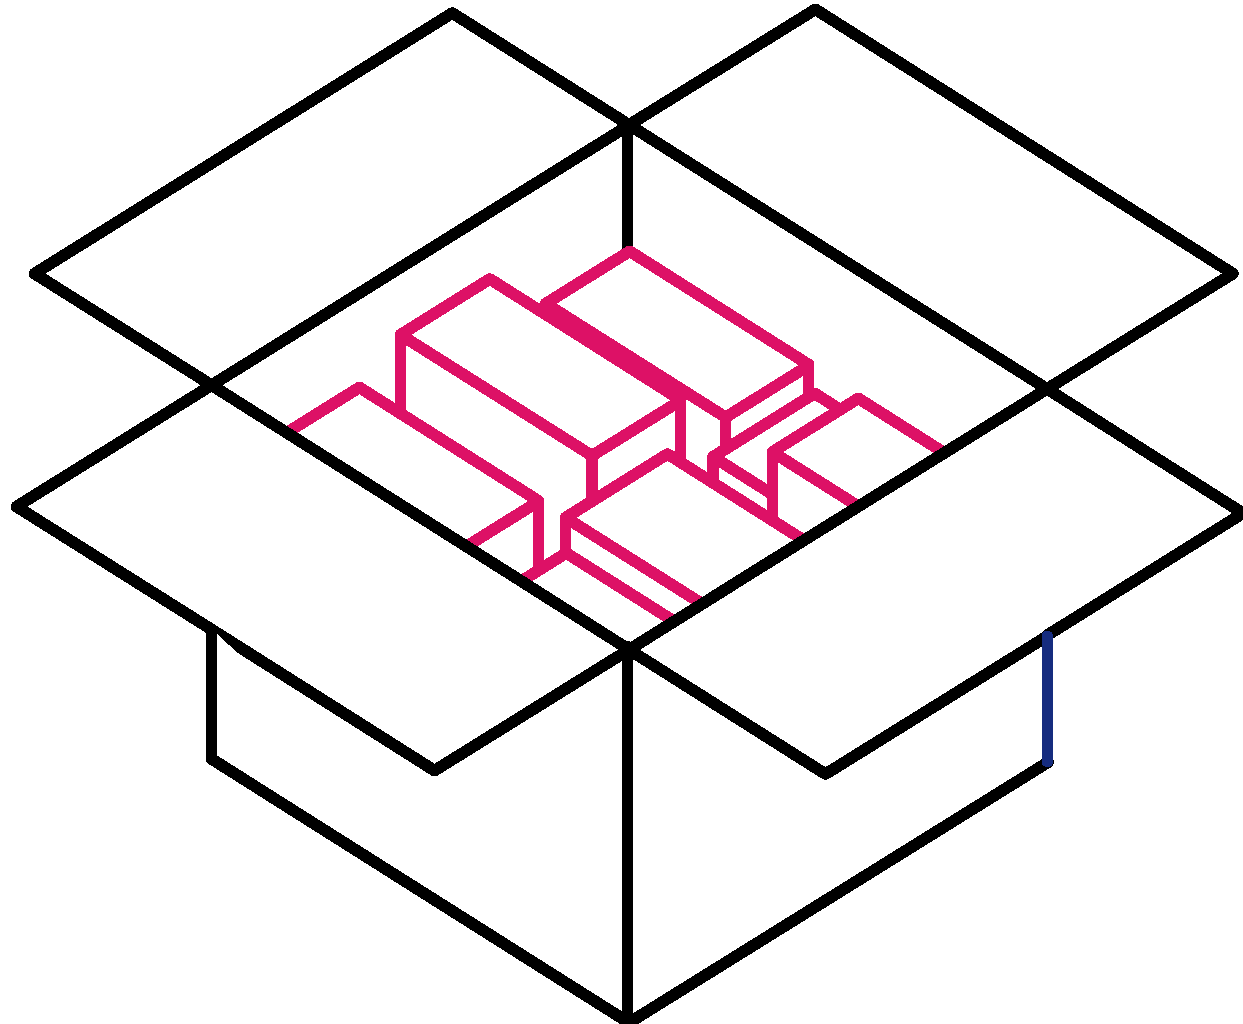
\includegraphics[height=20pt]{../assets/box.pdf}}
\rhead{} %Kopfzeile rechts
\lfoot{} %Fußzeile links
\cfoot{} %Fußzeile mitte
\rfoot{} %Fußzeile rechts
\makeatother


\newcommand{\changefont}{%
    \fontsize{9}{11}\selectfont
}


\setlength\headheight{60pt}
\setlength\footheight{40pt}
%\lfoot{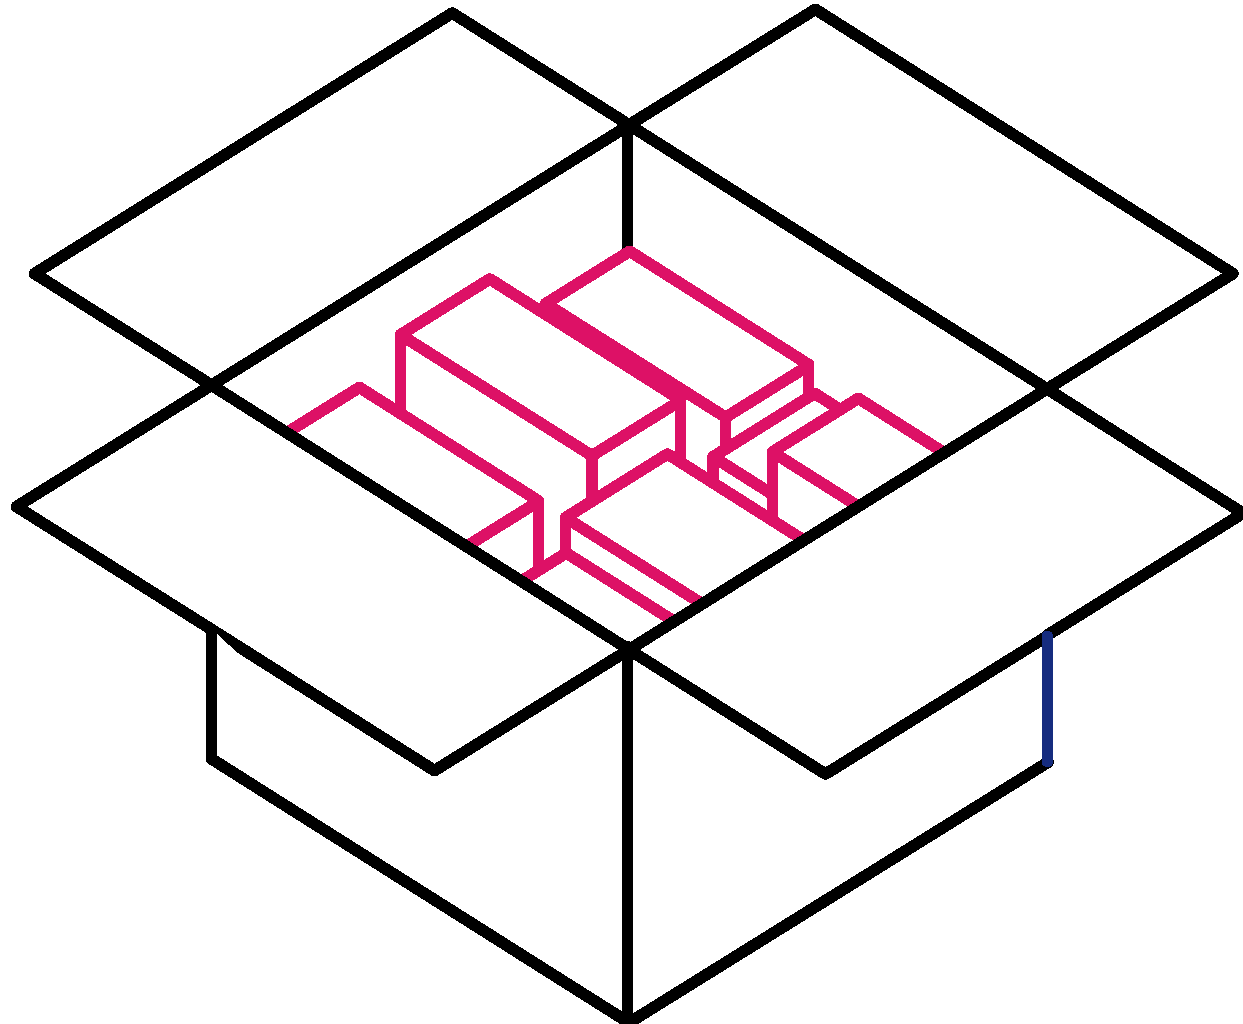
\includegraphics[height=40pt]{../assets/box.pdf}}
\rfoot{\thepage}
\lfoot{\changefont Selbstbericht Medieninformatik\\TH Köln // Institut für Informatik\\ \today}


%\UTF{0192}ndert die Seitennummerierung beim Inhaltsverzeichnis mit eigenem Stil
\renewcommand*{\indexpagestyle}{fancy}
%Verhindert die Seitennummerierung auf den Part-Seiten
\renewcommand*{\partpagestyle}{empty}
%\UTF{0192}ndert die Seitennummerierung bei Chapter mit eigenem Stil
\renewcommand*{\chapterpagestyle}{fancy}

%Abbildungsnummerierung ändern (abhängig von chapter, z.B. Abbildung 1.1)
\renewcommand*{\thefigure}{\thechapter.\arabic{figure}}
%Tabellennummerierung ändern (abhängig von chapter, z.B. Tabelle 1.1)
\renewcommand*{\thetable}{\thechapter.\arabic{table}}

%Paket, um ein Glossar/Abkürzungsverzeichnis anzulegen
\usepackage{nomencl}
\let\abbrev\nomenclature
%Der Name wird in Glossar geändert
\renewcommand{\nomname}{Glossar}
%Definiert die Aufteilung im Glossar zwischen Begriffen und Erläuterung
\setlength{\nomlabelwidth}{.25\hsize}
%Definiert die Punktelinien im Glossar
\renewcommand{\nomlabel}[1]{#1 \dotfill}
\setlength{\nomitemsep}{-\parsep}
%Veranlasst die Erstellung des Glossars
\makenomenclature

%Einrückungen nach Absätzen und Grafiken verhindern
\setlength{\parindent}{0pt}

%Verhindern, dass eine neue Seite für ein einzelnes Wort/Zeile verwendet wird
\clubpenalty = 10000 % schliesst Schusterjungen aus
\widowpenalty = 10000 % schliesst Hurenkinder aus (keine Beleidigung, sondern wirklich ein Fachbegriff)

%Paket für ein deutsches Literaturverzeichnis
\usepackage{bibgerm}

%Paket für die Verwendung von URLs durch den Befehl \url{}
%\usepackage{url}
\usepackage[hyphens]{url}

%Paket für Zeilenabstand (onehalfspace, singlespace)
\usepackage{setspace}

%Paket zur Erzeugung von Anführungszeichen durch \enquote{Text}
\usepackage[ngerman]{babel}
\usepackage[babel, german=quotes]{csquotes}

%Paket für farbigen Text
%black,white,green,red,blue,yellow,cyan,magenta
\usepackage{color}

%Paket für farbigen Hintergrund für Verbatim-Umgebung (Quelltext-Umgebung)
\usepackage{fancyvrb}
\usepackage{verbatim,moreverb}
%Grauton für Quelltext-Umgebung definieren 80% Grau
\definecolor{sourcegray}{gray}{.80}
%Paket für Quelltext-Umgebung
\usepackage{listings}

%Paket für Positionierung der Objekte ohne Float (Verwendungsbsp.: \begin{figure}[H])
\usepackage{float}

%Paket zur Erzeugung von Hyperrefs und PDF Informationen
\usepackage[pdftex,plainpages=false,pdfpagelabels,
            pdftitle={ Selbstbericht Medieninformatik // TH Köln // Institut für Informatik},
            pdfauthor={}
            ]{hyperref}
\hypersetup{
    colorlinks = true
}
\usepackage{pdfpages}

\providecommand{\tightlist}{%
  \setlength{\itemsep}{0pt}\setlength{\parskip}{0pt}}

\usepackage{tabularx}
\newcolumntype{L}[1]{>{\raggedright\arraybackslash}p{#1}}
\newcolumntype{C}[1]{>{\centering\arraybackslash}p{#1}}
\newcolumntype{R}[1]{>{\raggedleft\arraybackslash}p{#1}}

% URL
\PassOptionsToPackage{hyphens}{url}
\usepackage[pdftex]{hyperref}

% Sonderzeichen
\usepackage{textcomp}
\usepackage{eurosym}

\usepackage{setspace}
\renewcommand{\baselinestretch}{1.2}
\setlength{\parskip}{1em}

\usepackage[sfdefault,light]{roboto}  %% Option 'sfdefault' only if the base font of the document is to be sans serif


\usepackage[raggedright]{titlesec}
\titleformat{\chapter}[display]
  {\normalfont\sffamily\mdseries}
  {}{14pt}{\huge\raggedright}
% {\chaptertitlename\ \thechapter}{14pt}{\huge\raggedright}
\titleformat{\section}
  {\singlespacing\normalfont\sffamily\mdseries\Large\color{m_pink}\raggedright}
  {\thesection}{1em}{\Large}
\titleformat{\subsection}
  {\singlespacing\normalfont\sffamily\mdseries\large\raggedright}
  {\thesubsection}{1em}{\large}
% Zeilenumbruch und Spacing für Absätze
\titleformat{\paragraph}[hang]
  {\singlespacing\normalfont\normalsize\bfseries}
  {\theparagraph}{1em}{}
\titlespacing*{\paragraph}{0pt}{3.25ex plus 1ex minus .2ex}{0.5em}


\usepackage[font=footnotesize]{caption}


% Footer definieren
\makeatletter
\def\footrule{{
  \vskip-\footruleskip\vskip-\footrulewidth
  \color{\footrulecolor}
  \hrule\@width\headwidth\@height
  \footrulewidth\vskip\footruleskip
}}
\makeatother
\renewcommand{\footrulewidth}{0.1pt}
\newcommand{\footrulecolor}{m_green}



\begin{document}

%=== Deckblatt =======================================================
% Coversheet

\begin{titlepage}

	
\includegraphics[width=0.25\textwidth]{../../../assets/logo_th_koeln.pdf}

	\vspace{2cm}
	{\Huge\singlespacing\raggedright Modulhandbuch Medieninformatik Master\par}
	\vspace{1cm}
	{\Large TH Köln – Campus Gummersbach \\ Fakultät für Informatik und Ingenieurwissenschaften \\ Institut für Informatik\par}

	\vfill

% Bottom of the page
	{\large \today\par}
\end{titlepage}


%=== Inhaltsverzeichnis ==============================================
\tableofcontents

%=== Hauptteil =======================================================
%Seitennummerierung des Hauptteils
\mainmatter


\chapter{Auflagen zur
Akkreditierung\label{/mi-2017/selbstbericht/auflagen/0000-auflagen}}\label{auflagen-zur-akkreditierungpathlabelmi-2017selbstberichtauflagen0000-auflagen}

Die Akkreditierungskommission der ASIIN hat die Studiengänge
Medieninformatik Bachelor und Medieninformatik Master der TH Köln am 30.
Juni 2017 akkreditiert. Hierbei wurden einige Empfehlungen und Auflagen
formuliert. In diesem Dokument finden sich die Erläuterungen zur
fristgerechten Erfüllung der ausgesprochenen Auflagen.

\section{Auflagen für alle
Studiengänge\label{/mi-2017/selbstbericht/auflagen/0000-auflagen}}\label{auflagen-fuxfcr-alle-studienguxe4ngepathlabelmi-2017selbstberichtauflagen0000-auflagen}

\subsection{A1. (AR
2.3)\label{/mi-2017/selbstbericht/auflagen/0000-auflagen}}\label{a1.-ar-2.3pathlabelmi-2017selbstberichtauflagen0000-auflagen}

\begin{siderules}
Die Modulbeschreibungen müssen angemessen über die Voraussetzungen für
die Teilnahme, die Voraussetzungen für die Vergabe von Kreditpunkten und
Notenbildung sowie den Arbeitsaufwand informieren.
\end{siderules}

In den Modulbeschreibungen wurden die entsprechenden Angaben überprüft
und, soweit erforderlich, angepasst. Darüber hinaus wurde innerhalb der
Modulhandbücher jeweils eine kurze Einleitung an den Anfang gestellt.
Diese enthält einen graphischen Studienverlaufsplan, um insgesamt eine
bessere Verständlichkeit und Übersichtlichkeit herzustellen. Darüber
hinaus wurden Hyperlinks innerhalb der Handbücher farblich
hervorgehoben, um eine besser Handhabbarkeit und schnellere Navigation
im jeweiligen Handbuch zu ermöglichen.

Die aktuellen Modulhandbücher sind über folgende URL erreichbar:

\begin{itemize}
\tightlist
\item
  \href{http://www.medieninformatik.th-koeln.de/download/modulbeschreibungen-bachelor-bpo4.pdf}{Modulhandbuch
  Medieninformatik Bachelor}
\item
  \href{http://www.medieninformatik.th-koeln.de/download/modulbeschreibungen-master-mpo4.pdf}{Modulhandbuch
  Medieninformatik Master}
\end{itemize}

\subsection{A2. (AR 2.8)
\label{/mi-2017/selbstbericht/auflagen/0000-auflagen}}\label{a2.-ar-2.8-pathlabelmi-2017selbstberichtauflagen0000-auflagen}

\begin{siderules}
Die in Kraft gesetzten und veröffentlichten Ordnungen inklusive der
angepassten Diploma Supplements für beide Studiengänge sind vorzulegen.
\end{siderules}

Die Prüfungsordnung und der zugehörige Studienverlaufsplan für den
Medieninformatik Bachelor wurden mit der \textbf{Änderungssatzung vom
24.11.2017} in Kraft gesetzt und auf der Website der TH Köln
veröffentlicht:
\href{https://www.th-koeln.de/studium/medieninformatik-bachelor--ordnungen-und-formulare_3963.php}{Medieninformatik
(Bachelor) -- Ordnungen und Formulare}.

Hier findet sich ein Muster für das zugehörige
\href{https://th-koeln.github.io/mi-2017/download/auflagen/THK-DS-MIF-MIB-PO4.pdf}{Diploma
Supplement für den Medieninformatik Bachelor}

Die Prüfungsordnung und der zugehörige Studienverlaufsplan für den
Medieninformatik Master wurden mit der \textbf{Prüfungsordnung vom
13.07.2017} in Kraft gesetzt und auf der Website der TH Köln
veröffentlicht:
\href{https://www.th-koeln.de/studium/medieninformatik-master--ordnungen-und-formulare_3724.php}{Medieninformatik
(Master) -- Ordnungen und Formulare}.

Hier findet sich ein Muster für das zugehörige
\href{https://th-koeln.github.io/mi-2017/download/auflagen/THK-DS-MIF-MIM-PO4.pdf}{Diploma
Supplement für den Medieninformatik Master}.

Bitte beachten Sie, dass das Diploma Supplement auf speziellem Papier
gedruckt wird, auf dem ein Farbkeil (links) vorgedruckt ist, daher ist
dieser in der PDF-Datei nicht enthalten. Die mit ``«\ldots{}»''
gekennzeichneten Felder, werden bei Ausgabe mit den personalisierten
Daten der jeweiligen Absolvent*innen befüllt.

\section{Auflagen für den
Masterstudiengang\label{/mi-2017/selbstbericht/auflagen/0000-auflagen}}\label{auflagen-fuxfcr-den-masterstudiengangpathlabelmi-2017selbstberichtauflagen0000-auflagen}

\subsection{A3. (AR 2.1)
\label{/mi-2017/selbstbericht/auflagen/0000-auflagen}}\label{a3.-ar-2.1-pathlabelmi-2017selbstberichtauflagen0000-auflagen}

\begin{siderules}
Für die fünf Spezialisierungen des Masterstudiengangs ist eine
gleichmäßige detaillierte Beschreibung der Berufsfelder in den
Qualifikationszielen vorzunehmen. Die Module sind als eigenständige
Lehr-/Lerneinheiten darzustellen (unabhängig von der Darstellung der
Schwerpunkte, zu denen sie gehören).
\end{siderules}

Die Beschreibung der Spezialisierungen des Masterstudiengangs wurden im
Modulhandbuch um den Punkt «Berufsbilder» ergänzt. Aufgrund der
fachbedingten Unterschiede der Spezialisierungen, sind diese
Erläuterungen teilweise unterschiedlich aufgebaut, verfolgen aber alle
das Ziel, den Studierenden und Studieninteressierten klar zu machen,
welche beruflichen Perspektiven sich mit der jeweiligen Spezialisierung
eröffnen.

Die Schwerpunktspezifische Pflichtmodule der jeweiligen Spezialisierung
sind jetzt als farblich gekennzeichnete Hyperlinks im Handbuch
hinterlegt und führen direkt zur entsprechenden Modulbeschreibung des
jeweiligen Moduls. Die Modulbeschreibungen selbst, enthalten im
Factsheet zum Modul jetzt den Punkt «Pflichtmodul(e) im Schwerpunkt», um
die entsprechenden Zugehörigkeiten transparent zu machen.

Das überarbeitete Modulhandbucher ist über folgende URL erreichbar:

\begin{itemize}
\tightlist
\item
  \href{http://www.medieninformatik.th-koeln.de/download/modulbeschreibungen-master-mpo4.pdf}{Modulhandbuch
  Medieninformatik Master}
\end{itemize}

\begin{figure}[htbp]
\centering
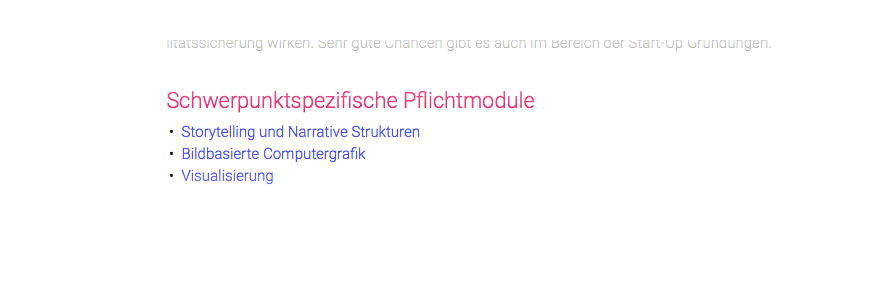
\includegraphics[width=\textwidth]{../anhaenge/bilder/hyperlinks.png}
\caption{Hyperlinks zu den Modulbeschreibungen}
\end{figure}

\begin{figure}[htbp]
\centering
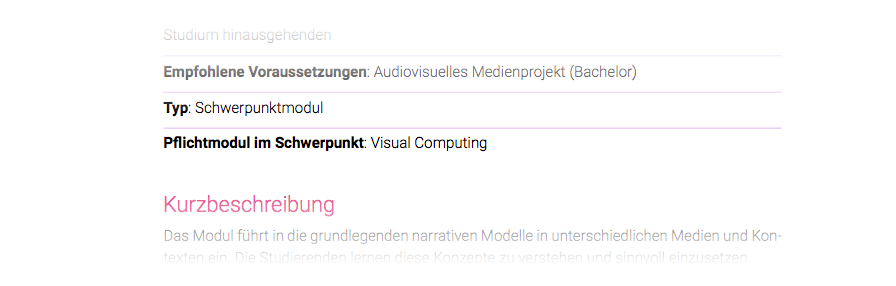
\includegraphics[width=\textwidth]{../anhaenge/bilder/pm-im-schwerpunkt.png}
\caption{Schwerpunktzugehörigkeit des jeweiligen Moduls}
\end{figure}


\begin{sloppypar}
\begin{flushleft}

\listoffootnotes

\end{flushleft}
\end{sloppypar}

\newpage

\listofattachments

\begin{sloppypar}
\begin{flushleft}

\begin{enumerate}
\item{Educational Diversity Konzept: \url{https://www.th-koeln.de/hochschule/educational-diversity\_5710.php} } 
\item{Forschungscluster: \url{https://www.th-koeln.de/forschung/cluster\_2734.php} } 
\item{Statistik Studierendenzahlen (01.12.2016): \url{https://th-koeln.github.io/mi-2017/anhaenge/stat-Studentenzahlen\_WS-2016\_(01.12.2016).pdf} } 
\item{Statistik zum Verbleib- und Studienabbruch: \url{https://th-koeln.github.io/mi-2017/anhaenge/stat-verbleib-und-studienabbruch.pdf} } 
\item{Hochschulentwicklungsplan 2020: \url{https://www.verwaltung.th-koeln.de/imperia/md/content/verwaltung/broschueren\_leitfaeden/hochschulentwicklungsplan2020.pdf} } 
\item{Ulrich Heublein et al.: Studienbereichsspezifische Qualitätssicherung im Bachelorstudium - Befragung der Fakultäts- und Fachbereichsleitungen zum Thema Studienerfolg und Studienabbruch. Forum Hochschule, 3/2015: \url{http://www.dzhw.eu/pdf/pub\_fh/fh-201503.pdf} } 
\item{Bachelorstudiengang Medieninformatik, Prüfungsstatistik 2016: \url{https://th-koeln.github.io/mi-2017/anhaenge/ba-pruefungsstatistiken.pdf} } 
\item{Fakultät für Informatik und Ingenieurwissenschaften, Statistik 2013/14: \url{https://th-koeln.github.io/mi-2017/anhaenge/fak-Fakultaetsstruktur-Studienangebot-Personal-Haushaltsmittel-Kennzahlen-2014.pdf} } 
\item{INCHER-Studie 2014: \url{https://th-koeln.github.io/mi-2017/anhaenge/studie-INCHER-Studie.pdf} } 
\item{Studentische Evaluationen Medieninformatik: \url{https://th-koeln.github.io/mi-2017/anhaenge/eva-evaluationen-f10.pdf} } 
\item{Curriculumsanalye: \url{https://th-koeln.github.io/mi-2017/anhaenge/ba-pruefungsstatistiken.pdf} } 
\item{Snapshot Bewertungen von studycheck.de: \url{https://th-koeln.github.io/mi-2017/anhaenge/eva-snapshot\_2017\_02\_17\_bewertungen\_studiengang\_medieninformatik\_auf\_studycheck\_.\_de.pdf} } 
\item{\url{http://studycheck.de}} 
\item{ProfiL2 Antrag der TH Köln: \url{https://www.th-koeln.de/mam/downloads/deutsch/hochschule/profil/lehre/profil2\_antrag\_ministerium.pdf} } 
\item{Studierendenbefragung 2010-2015: \url{https://th-koeln.github.io/mi-2017/anhaenge/eva-studierendenbefragung-2010-2015.pdf} } 
\item{Evaluation der studiengangsübergreifenden Module im Bachelor: \url{https://th-koeln.github.io/mi-2017/anhaenge/eva-lv-bewertung-mi-module-ba-kern.pdf} } 
\item{Evaluation der studiengangsspezifischen Module im Bachelor: \url{https://th-koeln.github.io/mi-2017/anhaenge/eva-lv-bewertung-mi-module-ba.pdf} } 
\item{Evaluation der studiengangsspezifischen Module im Master: \url{https://th-koeln.github.io/mi-2017/anhaenge/eva-lv-bewertung-mi-module-ma.pdf} } 
\item{Nachweis über ausreichende Lehrkapazität durch das Team 7.3(Personalcontrolling) der TH Köln: \url{https://th-koeln.github.io/mi-2017/anhaenge/th-verwaltung-kapa-nachweis.pdf} } 
\item{Wiederzuweisungsantrag des Instituts für Informatik (2013): \url{https://th-koeln.github.io/mi-2017/anhaenge/inst-AntragWiederzuweisung\_Motivation\_2013.pdf} } 
\item{Erläuterung zum Übereinkommen über die Anerkennung von Qualifikationen im Hochschulbereich in der europäischen Region: \url{https://de.wikipedia.org/wiki/\%C3\%9Cbereinkommen\_\%C3\%BCber\_die\_Anerkennung\_von\_Qualifikationen\_im\_Hochschulbereich\_in\_der\_europ\%C3\%A4ischen\_Region} } 
\item{Website des Medieninformatik Bachelor: \url{https://www.th-koeln.de/studium/medieninformatik-bachelor\_2379.php} } 
\item{Ordnungen zum Medieninformatik Bachelor: \url{https://www.th-koeln.de/studium/medieninformatik-bachelor--ordnungen-und-formulare\_3963.php} } 
\item{Themen der Abschlussabeiten des Medieninformatik Bachelor 2010 bis 2014: \url{https://th-koeln.github.io/mi-2017/anhaenge/ba-abschlussarbeiten\_2010-2014\_.pdf} } 
\item{Studienverlaufsplan Medieninformatik Bachelor: \url{https://th-koeln.github.io/mi-2017/anhaenge/ba-studienverlaufsplan.pdf} } 
\item{Modulhandbuch Medieninformatik Bachelor: \url{https://th-koeln.github.io/mi-2017/download/modulbeschreibungen-bachelor.pdf} } 
\item{Ziele-Module-Matrix Medieninformatik Bachelor: \url{https://th-koeln.github.io/mi-2017/anhaenge/ba-Ziele-Module-Matrix-Medieninformatik-Bachelor.pdf} } 
\item{Beispielzeugnis und Diploma Supplement Medieninformatik Bachelor: \url{https://th-koeln.github.io/mi-2017/anhaenge/ba-zeugnis.pdf} } 
\item{Profil der Studienanfänger: \url{https://th-koeln.github.io/mi-2017/anhaenge/stat-profil-studienanfaenger-2017.pdf} } 
\item{Website des Medieninformatik Master: \url{https://www.th-koeln.de/studium/medieninformatik-master\_3729.php} } 
\item{Ordnungen zum Medieninformatik Master: \url{https://www.th-koeln.de/studium/medieninformatik-master--ordnungen-und-formulare\_3724.php} } 
\item{Studienverlaufsplan Medieninformatik Master: \url{https://th-koeln.github.io/mi-2017/anhaenge/ma-studienverlaufsplan.pdf} } 
\item{Modulhandbuch Medieninformatik Master: \url{https://th-koeln.github.io/mi-2017/download/modulbeschreibungen-master.pdf} } 
\item{Prüfungsordnung Medieninformatik Master(entwurf): \url{https://th-koeln.github.io/mi-2017/anhaenge/ma-MIMPO\_Entwurf\_20170218.pdf} } 
\item{Ziele-Module-Matrix Medieninformatik Master: \url{https://th-koeln.github.io/mi-2017/anhaenge/ma-Ziele-Module-Matrix-Medieninformatik-Master.pdf} } 
\item{Beispielzeugnis und Diploma Supplement Medieninformatik Master: \url{https://th-koeln.github.io/mi-2017/anhaenge/ma-zeugnis.pdf} } 
\item{Empfehlungen für Bachelor- und Masterprogramme im Studienfach Informatik an Hochschulen: \url{https://www.gi.de/fileadmin/redaktion/empfehlungen/GI-Empfehlungen\_Bachelor-Master-Informatik2016.pdf} } 
\item{Medieninformatik 2016: Was war, was ist, was soll sein?: \url{http://dl.mensch-und-computer.de/bitstream/handle/123456789/5131/Kindsm\%C3\%BCller\_Wolters\_Heinecke\_2016.pdf} } 
\item{Studienverlaufsplan Medieninformatik Bachelor: \url{https://th-koeln.github.io/mi-2017/anhaenge/ba-studienverlaufsplan.pdf} } 
\item{Modulhandbuch Medieninformatik Bachelor: \url{https://th-koeln.github.io/mi-2017/download/modulbeschreibungen-bachelor.pdf} } 
\item{Ziele-Module-Matrix Medieninformatik Bachelor: \url{https://th-koeln.github.io/mi-2017/anhaenge/ba-Ziele-Module-Matrix-Medieninformatik-Bachelor.pdf} } 
\item{Beispielzeugnis und Diploma Supplement Medieninformatik Bachelor: \url{https://th-koeln.github.io/mi-2017/anhaenge/ba-zeugnis.pdf} } 
\item{Website des Medieninformatik Master: \url{https://www.th-koeln.de/studium/medieninformatik-master\_3729.php} } 
\item{Ordnungen zum Medieninformatik Master: \url{https://www.th-koeln.de/studium/medieninformatik-master--ordnungen-und-formulare\_3724.php} } 
\item{Studienverlaufsplan Medieninformatik Master: \url{https://th-koeln.github.io/mi-2017/anhaenge/ma-studienverlaufsplan.pdf} } 
\item{Modulhandbuch Medieninformatik Master: \url{https://th-koeln.github.io/mi-2017/download/modulbeschreibungen-master.pdf} } 
\item{Ziele-Module-Matrix Medieninformatik Master: \url{https://th-koeln.github.io/mi-2017/anhaenge/ma-Ziele-Module-Matrix-Medieninformatik-Master.pdf} } 
\item{Beispielzeugnis und Diploma Supplement Medieninformatik Master: \url{https://th-koeln.github.io/mi-2017/anhaenge/ma-zeugnis.pdf} } 
\item{Themen der Abschlussabeiten des Medieninformatik Bachelor 2010 bis 2014: \url{https://th-koeln.github.io/mi-2017/anhaenge/ba-abschlussarbeiten\_2010-2014\_.pdf} } 
\item{Studienverlaufsplan Medieninformatik Bachelor: \url{https://th-koeln.github.io/mi-2017/anhaenge/ba-studienverlaufsplan.pdf} } 
\item{Modulhandbuch Medieninformatik Bachelor: \url{https://th-koeln.github.io/mi-2017/download/modulbeschreibungen-bachelor.pdf} } 
\item{Ziele-Module-Matrix Medieninformatik Bachelor: \url{https://th-koeln.github.io/mi-2017/anhaenge/ba-Ziele-Module-Matrix-Medieninformatik-Bachelor.pdf} } 
\item{Beispielzeugnis und Diploma Supplement Medieninformatik Bachelor: \url{https://th-koeln.github.io/mi-2017/anhaenge/ba-zeugnis.pdf} } 
\item{Studienverlaufsplan Medieninformatik Master: \url{https://th-koeln.github.io/mi-2017/anhaenge/ma-studienverlaufsplan.pdf} } 
\item{Modulhandbuch Medieninformatik Master: \url{https://th-koeln.github.io/mi-2017/download/modulbeschreibungen-master.pdf} } 
\item{Prüfungsordnung Medieninformatik Master(entwurf): \url{https://th-koeln.github.io/mi-2017/anhaenge/ma-MIMPO\_Entwurf\_20170218.pdf} } 
\item{Ziele-Module-Matrix Medieninformatik Master: \url{https://th-koeln.github.io/mi-2017/anhaenge/ma-Ziele-Module-Matrix-Medieninformatik-Master.pdf} } 
\item{Beispielzeugnis und Diploma Supplement Medieninformatik Master: \url{https://th-koeln.github.io/mi-2017/anhaenge/ma-zeugnis.pdf} } 
\item{Profil der Studienanfänger: \url{https://th-koeln.github.io/mi-2017/anhaenge/stat-profil-studienanfaenger-2017.pdf} } 
\item{Homepage ProfiL2 Projektbörse: \url{http://projektboerse-profil2.th-koeln.de/} } 
\item{Fachbereich Mensch-Computer-Interaktion (MCI)/ Fachgruppe Medieninformatik: \url{http://fb-mci.gi.de/mensch-computer-interaktion-mci/fachgruppen/medieninformatik.html} } 
\item{Website International Office: \url{https://www.th-koeln.de/internationales/international-office\_1986.php} } 
\item{Prüfungsordnung Medieninformatik Bachelor: \url{https://www.th-koeln.de/studium/medieninformatik-bachelor--ordnungen-und-formulare\_3963.php} } 
\item{Prüfungsordnung Medieninformatik Master (Entwurf): \url{https://th-koeln.github.io/mi-2017/anhaenge/ma-MIMPO\_Entwurf\_20170218.pdf} } 
\item{Überblick über den Prüfungsprozess: \url{https://th-koeln.github.io/mi-2017/anhaenge/Prozessbeschreibung\_PruefungsprozessUeberblick.pdf} } 
\item{Prüfungsordnungsprozess: \url{https://th-koeln.github.io/mi-2017/anhaenge/Prozessbeschreibung\_Pruefungsordnungsprozess.pdf} } 
\item{Prozess zu Prüfungsplanung: \url{https://th-koeln.github.io/mi-2017/anhaenge/Prozessbeschreibung\_Pruefungplanung.pdf} } 
\item{Prozess zu Prüfunungsdurchführung: \url{https://th-koeln.github.io/mi-2017/anhaenge/Prozessbeschreibung\_Pruefungdurchfuehren.pdf} } 
\item{Prozess beim Rücktritt von Prüfungen: \url{https://th-koeln.github.io/mi-2017/anhaenge/Prozessbeschreibung\_vonPruefungzuruecktreten.pdf} } 
\item{Prozess beim Einspruch gegen Prüfungsergebnisse: \url{https://th-koeln.github.io/mi-2017/anhaenge/Prozessbeschreibung\_EinspruchPruefungsergebnisse.pdf} } 
\item{Prüfungsordnung Medieninformatik Bachelor: \url{https://www.th-koeln.de/studium/medieninformatik-bachelor--ordnungen-und-formulare\_3963.php} } 
\item{Studienverlaufsplan Medieninformatik Bachelor: \url{https://th-koeln.github.io/mi-2017/anhaenge/ba-studienverlaufsplan.pdf} } 
\item{Modulhandbuch Medieninformatik Bachelor: \url{https://th-koeln.github.io/mi-2017/download/modulbeschreibungen-bachelor.pdf} } 
\item{Prüfungsordnung Medieninformatik Master (Entwurf): \url{https://th-koeln.github.io/mi-2017/anhaenge/ma-MIMPO\_Entwurf\_20170218.pdf} } 
\item{Studienverlaufsplan Medieninformatik Master: \url{https://th-koeln.github.io/mi-2017/anhaenge/ma-studienverlaufsplan.pdf} } 
\item{Modulhandbuch Medieninformatik Master: \url{https://th-koeln.github.io/mi-2017/download/modulbeschreibungen-master.pdf} } 
\item{Beispielhafter Prüfungsplan: \url{https://th-koeln.github.io/mi-2017/anhaenge/ba-pruefungsplan\_mi.pdf} } 
\item{Analyse der Prüfungsteilnahme: \url{https://th-koeln.github.io/mi-2017/anhaenge/ba-pruefungsplan\_mi.pdf} } 
\item{Tabelle über Fehlversuche und Rücktritte: \url{https://th-koeln.github.io/mi-2017/anhaenge/ba-pruefungen-fehlversuche-und-ruecktritte.pdf} } 
\item{Personalhandbuch der des Instituts für Informatik: \url{http://bit.ly/2mpcbWN} } 
\item{Überblick über den Prüfungsprozess: \url{https://th-koeln.github.io/mi-2017/anhaenge/Prozessbeschreibung\_PruefungsprozessUeberblick.pdf} } 
\item{Prüfungsordnungsprozess: \url{https://th-koeln.github.io/mi-2017/anhaenge/Prozessbeschreibung\_Pruefungsordnungsprozess.pdf} } 
\item{Prozess zur Prüfungsplanung: \url{https://th-koeln.github.io/mi-2017/anhaenge/Prozessbeschreibung\_Pruefungplanung.pdf} } 
\item{Prozess zur Prüfunungsdurchführung: \url{https://th-koeln.github.io/mi-2017/anhaenge/Prozessbeschreibung\_Pruefungdurchfuehren.pdf} } 
\item{Prozess beim Rücktritt von Prüfungen: \url{https://th-koeln.github.io/mi-2017/anhaenge/Prozessbeschreibung\_vonPruefungzuruecktreten.pdf} } 
\item{Prozess beim Einspruch gegen Prüfungsergebnisse: \url{https://th-koeln.github.io/mi-2017/anhaenge/Prozessbeschreibung\_EinspruchPruefungsergebnisse.pdf} } 
\item{Prozess Absolventenzufriedenheit: \url{https://th-koeln.github.io/mi-2017/anhaenge/Prozessbeschreibung-Absolventenzufriedenheit.pdf} } 
\item{Prozess Evaluationsprozesse: \url{https://th-koeln.github.io/mi-2017/anhaenge/Prozessbeschreibung-Evaluationsprozesse.pdf} } 
\item{Prozess Partnerzufriedenheit: \url{https://th-koeln.github.io/mi-2017/anhaenge/Prozessbeschreibung-Partnerzufriedenheit.pdf} } 
\item{Prozess Rankings: \url{https://th-koeln.github.io/mi-2017/anhaenge/Prozessbeschreibung-Rankings.pdf} } 
\item{Prozess Studierendenzufriedenheit: \url{https://th-koeln.github.io/mi-2017/anhaenge/Prozessbeschreibung-Studierendenzufriedenheit.pdf} } 
\item{Gleichstellungskonzept der Technischen Hochschule Köln: \url{http://www.fh-koeln.de/mam/downloads/deutsch/hochschule/profil/gleichstellung/gleichstellungskonzept.pdf} } 
\item{Programm Educational Diversity der Technischen Hochschule Köln: \url{https://www.th-koeln.de/hochschule/educational-diversity\_5710.php} } 
\item{Profilseite zu Family Matters auf der Website der TH Köln: \url{https://www.th-koeln.de/hochschule/familienfreundlichkeit\_3759.php} } 
\item{Website: Studieren mit Beeinträchtigungen: \url{https://www.th-koeln.de/studium/studieren-mit-beeintraechtigung\_169.php} } 
\item{PDF: Studieren mit Beeinträchtigung - Handreichung für Lehrende und Beschäftigte der TH Köln. Zentrale Studienberatung, TH Köln, 2016: \url{https://www.th-koeln.de/mam/downloads/deutsch/studium/beratung/beeintraechtigung/a5brosch\_\_re\_beeintr\_\_chtigung\_2016.pdf} } 
\item{Übersicht über alle Mitarbeiter und deren Einbindung in die Kernmodule des Medieninformatik Bachelor Studiengangs am Campus Gummersbach: \url{https://th-koeln.github.io/mi-2017/anhaenge/stellungsnahme/mitarbeiter-und-module-mi-kern-2017.pdf} } 
\item{Übersicht über alle Dozenten und deren Module in den Informatik Studiengängen des Campus Gummersbach: \url{https://th-koeln.github.io/mi-2017/anhaenge/stellungsnahme/dozenten-und-module-2017.pdf} } 
\item{Zeugnismuster für die neue Studiengangsstruktur: \url{https://th-koeln.github.io/mi-2017/anhaenge/stellungsnahme/Urkunde\_Zeugnis\_Entwurf\_black.pdf} } 

\end{enumerate}

\end{flushleft}
\end{sloppypar}

%=== Schlussteil =====================================================
%%Seitennummerierung für den Anhang
\backmatter


\end{document}
